\documentclass{article}
\usepackage{amssymb}
\usepackage{amsmath}
\usepackage{empheq}
\usepackage{tcolorbox}
\usepackage[margin=2cm]{geometry}
\begin{document}
{\bf Problem}. Find roots of

\begin{equation}
  x^3+a_1x+a_0
  \label{eq:poly1}
\end{equation}

in exact form.

{\bf Solution} 

Case: $a_0, a_1 \in\mathbb{R}$

Attempt a solution of the form
\begin{equation}
  x=\sqrt[3]{g}+\sqrt[3]{h},
  \label{eq:trial1}
\end{equation}


After inserting $x$ as given in Eq. \eqref{eq:trial1} in Eq. \eqref{eq:poly1} we obtain

\begin{equation}
  g+h+3\sqrt{gh}\left(\sqrt[3]{g}+\sqrt[3]{h}\right)+a_1\left(\sqrt[3]{g}+\sqrt[3]{h}\right)+a_0=0
  \label{eq:sol1}
\end{equation}

Our goal is to eliminate the radix symbol from the algebra in \eqref{eq:sol1}. Therefore, we require:

\begin{equation}
  3\sqrt{gh}+a_1=0.
  \label{eq:req1}
\end{equation}

The requirement in \eqref{eq:req1} gives

\begin{equation}
  g=-\frac{a_1^3}{27h}
  \label{eq:g}
\end{equation}

and

\begin{equation}
  g+h+a_0=0.
  \label{eq:eq1}
\end{equation}

After substituting $g$ as given in Eqs. \eqref{eq:g} and \eqref{eq:eq1} and rearranging the terms we obtain a quadratic equation in $h$

\begin{equation}
  h^2+a_0h-\frac{a_1^3}{27}=0,
  \label{eq:eqh} 
\end{equation}

which is solved as:

\begin{equation}
  h_{1,2}=\frac{-a_0\pm\sqrt{a_0^2+\frac{4a_1^3}{27}}}{2}.
  \label{eq:solh}
\end{equation}

Together with Eq. \eqref{eq:g} (also $g=a_0-h$) we obtain one set of solutions:

\begin{equation}
  \begin{aligned}
    h=\frac{-a_0+\sqrt{a_0^2+\frac{4a_1^3}{27}}}{2}, \quad & g=\frac{-a_0-\sqrt{a_0^2+\frac{4a_1^3}{27}}}{2} 
  \end{aligned}
\end{equation}

and

\begin{equation}
  x_1=\sqrt[3]{\frac{-a_0-\sqrt{a_0^2+\frac{4a_1^3}{27}}}{2}}+\sqrt[3]{\frac{-a_0+\sqrt{a_0^2+\frac{4a_1^3}{27}}}{2}}.
\end{equation}

One can observe that $x_1=\sqrt[3]{k_1}+\sqrt[3]{k_2}$, where $k_{1,2}$ are the roots of the equation $k^2+a_0k-\frac{a_1^{3}}{27}=0$.

Let us denote the discriminant $a_0^2+\frac{4a_1^3}{27}$ as $D$.

Now we are left with the task of finding the other two roots $x_1$ and $x_2$. This is a simpler task because now we handle a quadratic polynomial, and standard high-school textbooks show how to calculate the roots of such a polynomial.

Given that the polynomial in Eq. \eqref{eq:poly1} can be expressed as

\begin{equation}
  \left(x-x_1\right)\left(x-x_2\right)\left(x-x_3\right)=0
\end{equation}

we can work with the equations for the coefficients $a_1$ and $a_0$

\begin{equation}
  a_1=x_1x_2+x_2x_3+x_3x_1,
\end{equation}

\begin{equation}
  a_0=-x_1x_2x_3.
\end{equation}

Solving them for $x_2$ we obtain an equation:

\begin{equation}
  x_1^2x_2^2-a_0x_1+x_3^4=0.
\end{equation}

By solving for $x$ and simplifying we obtain:

\begin{equation}
  x_2=\frac{-x_1+\sqrt{-3\left(x_1^2-4a_1\right)}}{2}.
\end{equation}

This solution can also be obtained by dividing the original polynomial in \eqref{eq:poly1} with $\left(x-x_1\right)$ and finding the roots of the resulting quadratic polynomial. 

Since $a_1=-3\sqrt[3]{gh}$ it can be shown that

\begin{equation}
  -3\left(x_1^2-4a_1\right)=-3\left(\sqrt{g}-\sqrt{h}\right)^2.
\end{equation}

Thus we obtain the solutions:

\begin{align}
  x_1 &= \sqrt[3]{g}+\sqrt[3]{h}  \label{eq:solx1gen}\\
  x_2 &= \frac{-\sqrt[3]{g}-\sqrt[3]{h}+i\sqrt{3}\left(\sqrt[3]{g}-\sqrt[3]{h}\right)}{2} \label{eq:solx2gen}\\
  x_3 &= \frac{-\sqrt[3]{g}-\sqrt[3]{h}-i\sqrt{3}\left(\sqrt[3]{g}-\sqrt[3]{h}\right)}{2} \label{eq:solx3gen},  
\end{align}

or

\begin{align}
  x_1 &= \sqrt[3]{g}+\sqrt[3]{h} \\
  x_2 &= \frac{\sqrt[3]{h}\left(-1-\sqrt{3}i\right)+\sqrt[3]{g}\left(-1+\sqrt{3}i\right)}{2} \\
  x_3 &= \frac{\sqrt[3]{h}\left(-1+\sqrt{3}i\right)+\sqrt[3]{g}\left(-1-\sqrt{3}i\right)}{2}.
  \label{eq:solDgeq01}
\end{align}

The solution becomes more illuminating after we recognise that $-1+\sqrt{3}i=e^{\frac{2\pi i}{3}}$ and $-1-\sqrt{3}i=e^{\frac{4\pi i}{3}}$, see Fig. \ref{fig:complexphases}. Furthermore, $e^{\frac{4\pi i}{3}}=e^{-\frac{2\pi i}{3}}$. Hence the roots can be written in the form shown in Eqs \eqref{eq:solDgeq02x1}, \eqref{eq:solDgeq02x2} and  \eqref{eq:solDgeq02x3}:

\begin{figure}
  \centering
  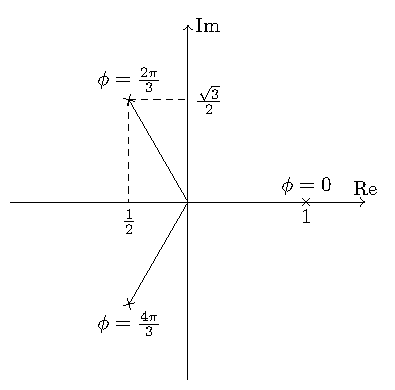
\includegraphics[width=0.5\textwidth]{Figures/complexphaseplot}
  \caption{$e^{i0}$, $e{^\frac{2\pi i}{3}}$, $e{^\frac{4\pi i}{3}}$ plotted on the complex plane} 
  \label{fig:complexphases}
\end{figure}

\begin{tcolorbox}
  For $a_0$ and $D\in\mathbb{R}$ and $D\geq0$:
  \begin{empheq}[box=\fbox]{align}
    x_1 &= \sqrt[3]{g}+\sqrt[3]{h} \label{eq:solDgeq02x1}\\
    x_2 &= \sqrt[3]{h}e^{\frac{-2\pi i}{3}}+\sqrt[3]{g}e^{\frac{2\pi i}{3}} \label{eq:solDgeq02x2} \\
    x_3 &= \sqrt[3]{h}e^{\frac{2\pi i}{3}}+\sqrt[3]{g}e^{-\frac{2\pi i}{3}} \label{eq:solDgeq02x3}
  \end{empheq}

  where 
  \begin{equation}
    \begin{aligned}
      h=\frac{-a_0+\sqrt{D}}{2}, \quad & g=\frac{-a_0-\sqrt{D}}{2} 
    \end{aligned}
  \end{equation}

  and

  \begin{equation}
    D=a_0^2+\frac{4a_1^3}{27}.
  \end{equation}
\end{tcolorbox}

In the case $a_0\in\mathbb{R}$ and $D=0$ there are two equal roots:

\begin{tcolorbox}
  For $a_0\in\mathbb{R}$ and $D=0$:
 \begin{empheq}[box=\fbox]{align}
   g=h=-\frac{a_0}{2}.
 \end{empheq}
 
 \begin{empheq}[box=\fbox]{align}
   &x_1=-2\sqrt[3]{\frac{a_0}{2}}\\
   &x_2=x_3=\sqrt[3]{\frac{a_0}{2}}.
 \end{empheq}

\end{tcolorbox}

For the case $a_0,D_0\in\mathbb{R}$ and $D<0$ we observe that:

\begin{align}
  |g|=|h|=\frac{-a_1}{3},\\
  \sqrt[3]{h}=\sqrt[2]{\frac{-a_1}{3}}e^{\frac{i\phi_h}{3}},\\
  \sqrt[3]{g}=\sqrt[2]{\frac{-a_1}{3}}e^{\frac{-i\phi_h}{3}},
\end{align}

\begin{align}
  \sqrt[3]{h}+\sqrt[3]{g}&=2\sqrt{\frac{-a_1}{3}}\cos\left(\frac{\phi_h}{3}\right),\\ 
  \sqrt[3]{h}-\sqrt[3]{g}&=2i\sqrt{\frac{-a_1}{3}}\sin\left(\frac{\phi_h}{3}\right). 
\end{align}

where $\phi_h$ is the phase of $h$ (see \eqref{eq:phi_h}).

Therefore,
\begin{align}
  x_1&=2\sqrt{\frac{-a_1}{3}}\cos\left(\frac{\phi_h}{3}\right),\\ 
  x_2&=\sqrt{\frac{-a_1}{3}}\left(-\cos\left(\frac{\phi_h}{3}\right)+\sqrt{3}\sin\left(\frac{\phi_h}{3}\right)\right),\\
  x_3&=\sqrt{\frac{-a_1}{3}}\left(-\cos\left(\frac{\phi_h}{3}\right)-\sqrt{3}\sin\left(\frac{\phi_h}{3}\right)\right). 
\end{align}

By noting that (see Fig. \ref{fig:angles_polar})
\begin{align}
  \cos\left(\frac{2\pi}{3}\right)&=-\frac{1}{2} & \sin\left(\frac{2\pi}{3}\right)&=\frac{\sqrt{3}}{2}\\
  \cos\left(\frac{4\pi}{3}\right)&=-\frac{1}{2} & \sin\left(\frac{4\pi}{3}\right)&=-\frac{\sqrt{3}}{2}
\end{align}

$x_2$ and $x_3$ can be expressed as 


\begin{align}
  x_2&=2\sqrt{\frac{-a_1}{3}}\left(\cos\left(\frac{2\pi}{3}\right)\cos\left(\frac{\phi_h}{3}\right)+\sin\left(\frac{2\pi}{3}\right)\sin\left(\frac{\phi_h}{3}\right)\right),\\
  x_3&=2\sqrt{\frac{-a_1}{3}}\left(\cos\left(\frac{4\pi}{3}\right)\cos\left(\frac{\phi_h}{3}\right)+\sin\left(\frac{4\pi}{3}\right)\sin\left(\frac{\phi_h}{3}\right)\right).
\end{align}

\begin{figure}
  \centering
  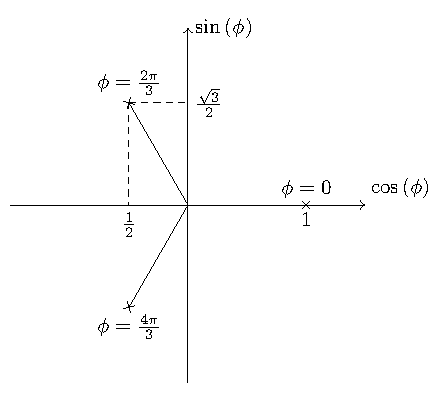
\includegraphics[width=0.5\textwidth]{Figures/angles}
  \caption{$\phi=0\text{,}\ \frac{2\pi}{3}\text{,}\ \frac{4\pi}{3}$ plotted in polar coordinates}
  \label{fig:angles_polar}
\end{figure}

By using the relationship

\begin{equation}
  \cos\left(\alpha+\beta\right)=\cos\left(\alpha\right)\cos\left(\beta\right)-\sin\left(\alpha\right)\sin\left(\beta\right)
\end{equation}

the roots can be recast in a more illuminating form as given in equations \eqref{eq:solDlessthan0x1}, \eqref{eq:solDlessthan0x2}, \eqref{eq:solDlessthan0x3}. 
\begin{tcolorbox}
  For $a_0$ and $D\in\mathbb{R}$ and $D<0$:
  \begin{empheq}[box=\fbox]{align}
    x_1 &= 2\sqrt{-\frac{a_1}{3}}\cos\left(\frac{\phi_h}{3}\right), \label{eq:solDlessthan0x1}\\
    x_2 &= 2\sqrt{-\frac{a_1}{3}}\cos\left(\frac{\phi_h}{3}-\frac{2\pi}{3}\right), \label{eq:solDlessthan0x2}\\    
    x_3 &= 2\sqrt{-\frac{a_1}{3}}\cos\left(\frac{\phi_h}{3}+\frac{2\pi}{3}\right). \label{eq:solDlessthan0x3}
  \end{empheq}

  where 
  \begin{equation}
    \begin{aligned}
      h=\frac{-a_0+i\sqrt{-D}}{2}, \quad & g=\frac{-a_0-i\sqrt{-D}}{2} 
    \end{aligned}
  \end{equation}

  and

  \begin{equation}
    D=a_0^2+\frac{4a_1^3}{27},
  \end{equation}

  and the phase $\phi_h$ is taken with respect to $h$ and is calculated as

  \begin{align}
    \phi_h &= \arctan\left(\frac{\sqrt{-D}}{-a_0}\right)+n\pi,\quad \text{where } n=0 \quad \text{if } a_0<0,\quad n=1\quad\text{if } a_0>0 \\
    &= \frac{\pi}{2},\quad \text{if } a_0=0
    \label{eq:phi_h}
  \end{align}
  
\end{tcolorbox}

From equations \eqref{eq:solDlessthan0x1}, \eqref{eq:solDlessthan0x2}, \eqref{eq:solDlessthan0x3} it can be seen that the roots follow each other by phase $\frac{2\pi}{3}$ in the sequence $x_2\text{---} x_1\text{---} x_3$.

Eqs. \eqref{eq:solDlessthan0x1}, \eqref{eq:solDlessthan0x2}, \eqref{eq:solDlessthan0x3} are generators of interesting identities. For example, trying the roots $-1, -2, 3$, we find that:
\begin{equation}
  3=2\sqrt{\frac{7}{3}}\cos\left(\frac{1}{3}\arctan\left(\frac{10}{9\sqrt{3}}\right)\right)
\end{equation}

Now, we would like to develop the general solution for the case $a_0, a_1 \in \mathbb{C}$, $a_1\neq0$. We consider $g$ and $h$ as complex numbers:
\begin{align}
  g&=|g|e^{\left(i\left(\phi_g+n_g2\pi\right)\right)},\\
  h&=|h|e^{\left(i\left(\phi_h+n_h2\pi\right)\right)},\\
\end{align}
where $n_g$ are $n_h$ integers. While $g$ and $h$ have equal values for all $n_g$ and $n_h$ respectively, the roots of $g$ and $h$ don't as we will see shortly. From the requirement \eqref{eq:req1} it follows that

\begin{equation}
  3\sqrt[3]{|g||h|}e^\frac{i\left(\phi_g+\phi_h+\left(n_g+n_h\right)2\pi\right)}{3}=|a_1|e^{i\left(\phi_a+\pi\right)}.
\end{equation}

Hence

\begin{equation}
  n_h+n_g=\frac{3\left(\phi_a+\pi\right)-\phi_g-\phi_h}{2\pi}
  \label{eq:n_hn_g}.
\end{equation}

We note the gauge freedom \textendash $n_h$ and $n_g$ can be any real integer, only their sum must satisfy Eq. \eqref{eq:n_hn_g}.

After cubing both sides of the equation \eqref{eq:req1} we obtain:

\begin{equation}
  |g|e^{i\phi_g}=-\frac{a_1^{3}}{27|h|e^{i\phi_h}}
\end{equation}

and

\begin{equation}
  \left(|h|e^{i\phi_h}\right)^2+a_0|h|e^{i\phi_h}+a_0=0.
\end{equation}

We obtain the $g$ and $h$ solutions

\begin{align}
  |h|e^{i\phi_h}&=\frac{-a_0+\sqrt{D}}{2},\\
  |g|e^{i\phi_h}&=\frac{-a_0-\sqrt{D}}{2}
\end{align}

From \eqref{eq:solx1gen}, \eqref{eq:solx2gen} and \eqref{eq:solx3gen} we obtain

\begin{equation}
  x_1=\sqrt[3]{|h|}e^{\frac{i\left(\phi_h+n_h2\pi\right)}{3}}+\sqrt[3]{|g|}e^{\frac{i\left(\phi_g+n_g2\pi\right)}{3}}
\end{equation}

\begin{equation}
  x_2=\frac{
    \sqrt[3]{|h|}
    e^{
      \frac{i\left(\phi_h+n_h2\pi\right)}{3}
    }
    \left(-1-\sqrt{3}i\right)+
    \sqrt[3]{|g|}e^{
      \frac{i\left(\phi_g+n_g2\pi\right)}{3}
      }
    \left(-1+\sqrt{3}i\right)
    }{2}
\end{equation}

\begin{equation}
  x_3=\frac{
    \sqrt[3]{|h|}
    e^{
      \frac{i\left(\phi_h+n_h2\pi\right)}{3}
    }
    \left(-1+\sqrt{3}i\right)+
    \sqrt[3]{|g|}e^{
      \frac{i\left(\phi_g+n_g2\pi\right)}{3}
      }
    \left(-1-\sqrt{3}i\right)
    }{2}
\end{equation}

After simplifying, we obtain the following:

\begin{tcolorbox}
  For $a_0$ and $D\in\mathbb{C}$ and $a_1\neq0$:
  \begin{empheq}[box=\fbox]{align}
    x_1 &= \sqrt[3]{|h|}e^{\frac{i\left(\phi_h+n_h2\pi\right)}{3}}+\sqrt[3]{|g|}e^{\frac{i\left(\phi_g+n_g2\pi\right)}{3}}, \\
    x_2 &= \sqrt[3]{|h|}e^{\frac{i\left(\phi_h+n_h2\pi\right)}{3}-\frac{2\pi i}{3}}+\sqrt[3]{|g|}e^{\frac{i\left(\phi_g+n_g2\pi\right)}{3}+\frac{2\pi i}{3}}, \\
    x_3 &= \sqrt[3]{|h|}e^{\frac{i\left(\phi_h+n_h2\pi\right)}{3}+\frac{2\pi i}{3}}+\sqrt[3]{|g|}e^{\frac{i\left(\phi_g+n_g2\pi\right)}{3}-\frac{2\pi i}{3}},
  \end{empheq}

  where 
  \begin{equation}
    \begin{aligned}
      h=\frac{-a_0+\sqrt{D}}{2}, \quad & g=\frac{-a_0-\sqrt{D}}{2} 
    \end{aligned}
  \end{equation}

  and

  \begin{equation}
    D=a_0^2+\frac{4a_1^3}{27}.
  \end{equation}
  
  \begin{equation}
    n_h+n_g=\frac{3\left(\phi_a+\pi\right)-\phi_g-\phi_h}{2\pi}
  \end{equation}

  and the phase

  
  \begin{align}
    \phi_f &= \arctan\left(\frac{i\left(f^*-f\right)}{f+f^*}\right)+n\pi,\quad \text{where } n=0 \quad \text{if } f+f^*>0,\quad n=1\quad\text{if } f+f^*<0 \\
    &= \frac{\pi}{2},\quad \text{if } a_0=0\quad \text{and}\quad i\left(f^*-f\right)>0,\\
    &= \frac{3\pi}{2},\quad \text{if } a_0=0\quad \text{and}\quad i\left(f^*-f\right)<0,
    \label{eq:phi_h}
  \end{align}

  where $f^*$ denotes the complex conjugate of f.
  
\end{tcolorbox}


The general solution is depicted in tgee Argand diagram in Figure~\ref{fig:generalsolution}, where we have introduced new variables for convenience:

\begin{align}
  H&=\sqrt[3]{h}e^{i\left(\frac{\phi_h}{3}+\frac{n_h2\pi}{3}\right)},\\
  G&=\sqrt[3]{g}e^{i\left(\frac{\phi_g}{3}+\frac{n_g2\pi}{3}\right)}.
\end{align}

\begin{figure}
  \centering
  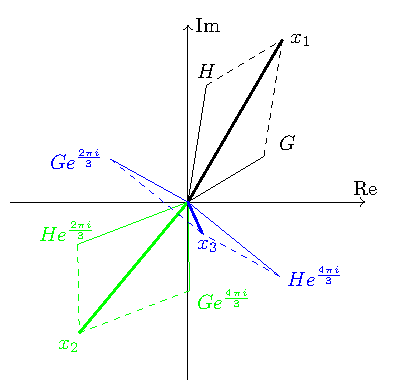
\includegraphics[width=0.5\textwidth]{Figures/generalsolution.pdf}
  \caption{Argand diagram of a general solution}
  \label{fig:generalsolution}
\end{figure}

In the case of $a_1=0$ we cannot use the solution for $a_1\neq0$ because the phase of $a_1$ is not defined. In this case $h=0$ and $g=|a_0|e^{\pi i}$. By plugging in these values in Eqs. \eqref{eq:solDgeq02x1}, \eqref{eq:solDgeq02x2} and \eqref{eq:solDgeq02x3} we obtain the following roots:

\begin{tcolorbox}
  For $a_0$ and $D\in\mathbb{R}$ and $D\geq0$:
  \begin{empheq}[box=\fbox]{align}
    x_1 &= \sqrt[3]{|a_0|}e^{\frac{\left(\phi_{a_0}+\pi \right)i}{3}},\\
    x_2 &= \sqrt[3]{|a_0|}e^{\frac{\left(\phi_{a_0}+5\pi \right)i}{3}},\\
    x_3 &= -\sqrt[3]{|a_0|}e^{\frac{\phi_{a_0}i}{3}}.
  \end{empheq}
\end{tcolorbox}

In the case $a_0=0$, $\sqrt[3]{g}=-\sqrt{\frac{a_1}{3}}$, $\sqrt[3]{h}=\sqrt{\frac{a_1}{3}}$ the following solutions are obtained:

\begin{tcolorbox}
  If $a_0=0$:
  \begin{empheq}[box=\fbox]{align}
    x_1 &= 0,\\
    x_2 &= i\sqrt{|a_1|}e^{i\phi_{a_1}}\\
    x_3 &= -i\sqrt{|a_1|}e^{i\phi_{a_1}}.
  \end{empheq}
\end{tcolorbox}

{\bf General case}

We want to find the solutions of the equation

\begin{equation}
  b_3x^3+b_2x^2+b_1x+b_0=0.
\end{equation}

We introduce the substitution $x=x'+p$ and obtain:

\begin{equation}
  b_3x'^3+\left(3b_3p+b_2\right)x'^2+\left(3b^3p^2+2pb_2+b_1\right)x'+b_3p^3+b_2p^2+b_1p+b_0=0.
  \label{eq:gen_eq}
\end{equation}

We require the $x^{'2}$ term to vanish, hence:

\begin{equation}
  p=-\frac{b_2}{3b_3}.
  \label{eq:p}
\end{equation}

From Eqs. \eqref{eq:gen_eq} and \eqref{eq:p} we obtain the coefficients $a_0$ and $a_1$ in Eq. \eqref{eq:poly1}:

\begin{equation}
  a_1=\frac{1}{b_3}\left(-\frac{b_2^3}{3b_3}+b_1\right),
\end{equation}

\begin{equation}
  a_0=\frac{1}{b_3}\left(\frac{b_2^3}{27b_3^2}-\frac{b_1b_2}{3b_3}+b_0\right).
\end{equation}

Subsequently, we find the roots of the polynomial of $x'$ in Eq. \eqref{eq:poly1}, and afterwards transform $x=x'+p$.

\end{document}

